\section{Introduction}
\seclabel{introduction}

Consider the chairs in \figref{fig1}. As humans, not only can we infer at a glance that the image contains three chairs, we also construct a rich internal representation of each of them such as their locations and 3D poses. Moreover, we have a guess of their 3D shapes, even though we might never have seen these particular chairs. We can do this because we do not experience this image {\em tabula rasa}, but in the context of our  ``remembrance of things past".   Previously seen chairs enable us to develop a notion of the 3D shape of chairs, which we can project to the instances in this particular image. We also specialize our representation to these particular instances (e.g. any custom decorations they might have), signalling that both top-down and bottom-up cues influence our percept~\cite{nandakumar2011little}. In this work, we incorporate these principles in a computational framewoek for reconstructing objects given a single image. 

The task of reconstructing objects from a single image is a challenging one -- a typical image depicts many objects, each possibly belonging to a different object category; an object category, in turn, comprises instances of varying shapes, textures, size \etc and any particular instance may be viewed from a different viewpoint. Previous approaches to this problem can be broadly grouped into two paradigms. The paradigm of model-based object reconstruction has reflected varying preferences on model representations.  Generalized cylinders~\cite{nevatia1977description} resulted in very compact descriptions for certain classes of shapes, and can be used for category level descriptions, but the fitting problem for general shapes is challenging. Polyhedral models~\cite{gupta2010blocks,xiao2012localizing}, which trace back to the early work of Roberts \cite{roberts1963machine}, and CAD models~\cite{limparsing,satkin20143dnn,Pepik_2015_CVPR_Workshops}, cannot perfectly deform into shapes even slightly different from those in training data, but given a set of point correspondences can be quite effective for determining approximate instance viewpoints. Some recent methods have proposed using similar instances from a collection of CAD models \cite{su2014estimating,huang2015single} for  non-parametric reconstruction but their applications have been restricted to pre-segmented online product images or recovering 3D from 2.5D object scans~\cite{sung2015data}. Here we pursue more expressive basis shape models~\cite{Anguelov:SCAPE2005,blanz1999morphable,zia2013detailed} which establish a balance between the two extremes as they can deform but only along class-specific modes of variation.

\begin{figure}[t]
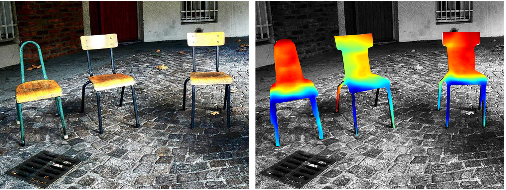
\includegraphics[width = \textwidth]{figures/categoryshapes/teaserChair.pdf}
\caption{Example outputs of our system, given a single image of a scene having chairs, a class that the system was exposed to during training. The coloring on the right image signals object-centric depth (we do not aim for globally consistent depths across multiple objects). Blue means close to the camera, red means far from the camera.}
  \figlabel{fig1}
\end{figure}

The alternate paradigm comprises of approaches that target the problem of object reconstruction in a class or object agnostic manner, either implicitly or explicitly using generic learned 3D shape cues \cite{hoiem2005automatic, saxena2009make3d}, or bottom-up cues and the physics of image formation \cite{Karsch2013,barronPAMI13} building upon the long tradition of shape-from-X, which traces back to seminal work by Horn \cite{HORNThesis1970}. These methods, while quite general, have not yet been demonstrated for 3D reconstruction -- as opposed to 2.5D -- and typically assume known object segmentation \cite{barronPAMI13}. Some recent approaches have demonstrated the use of supervised learning techniques to implcitly learn generic cues to predict depth maps \cite{eigennips14} and surface normals \cite{eigen2015predicting, wang2015designing} but these have primarily focused on  inferring scene-level information which differs from our goal of perceiving the shape of objects.

In this work, we combine both these reconstruction paradigms - we obtain top-down shape information from our model-based reconstruction approach and complement it with bottom-up shape information obtained via an intrinsic image decomposition method.  Crucially, in contrast to previous work (e.g. \cite{barronPAMI13,carvi14,cashman2013dolphins}), we do not require perfect knowledge of object localization and pose as our reconstruction is driven by automatic figure-ground object segmentations and viewpoint estimations.

\begin{figure}[t]
\centering
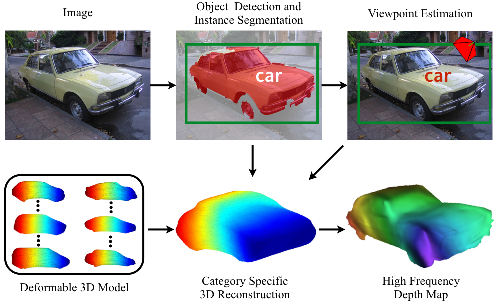
\includegraphics[width = .9\textwidth]{figures/categoryshapes/figTest.pdf}
\caption{Overview of our full reconstruction method. We leverage estimated instance segmentations and predicted viewpoints to generate a full 3D mesh and a high frequency 2.5D depth map for each object in the image.}
\figlabel{figTest}
\end{figure}

The framework we propose to reconstruct the objects present in an image is outlined in \figref{figTest}. As a first step, we leverage the recent progress made by the computer vision community in object detection ~\cite{rcnn} and instance segmentation~\cite{BharathECCV2014, BharathCVPR2015} to identify and localize objects in the image. For each object, we also predict a viewpoint in the form of three euler angles. We then use our learned deformable 3D shape models in conjunction with the viewpoint and localization information to produce a ``top-down'' 3D reconstruction for the object guided primarily by category level cues. Finally, we infuse our 3D shape with high frequency local shape cues to obtain our end result - a rich 3D reconstruction of the object. We briefly outline each of the components required for the above proposed framework.

\paragraph{Learning Deformable 3D Models.}
As noted earlier, previously seen objects allow us to develop a notion of 3D shape which informs inference for new instances. We present an algorithm that can build category-specific  deformable shape models from just images with 2D annotations (segmentation masks and a small set of keypoints) present in modern computer vision datasets (e.g. PASCAL VOC~\cite{pascal-voc-2012}). These learnt shape models and deformations allow us to robustly infer shape while capturing intra-class shape variation.

\paragraph{Learning to Estimate Viewpoint.}
The first step towards being able to represent objects in 3D is to predict their viewpoint. This intermediate representation provides coarse information about the shape and its inference is a well studied problem in computer vision \cite{huttenlocher1990recognizing, rothganger20063d, gordon2006and, savarese2008view, xiao2008structuring, gu2010discriminative, ozuysal2009pose}.
We train a Convolutional Neural Network (CNN) ~\cite{neocognitron,LeCun1989} based architecture which can implicitly capture and aggregate local evidence to obtain a viewpoint estimate and demonstrate improvements over the state-of-the-art for this task.

\paragraph{Object Shape Recovery.}
Given an object's category, approximate localization and viewpoint, we obtain a 3D reconstruction for the corresponding object using the learned category-specific deformable shape model. We complement the top-down shape inferred via this inference with a bottom-up module that further refines our shape estimate for a particular instance. This framework allows us to capture the coarse as well as fine level shape details for objects from a single image.

Our paper is organized as follows: in \secref{modelLearning} we describe our model learning pipeline where we estimate camera parameters for all training objects (\secref{nrsfm}) followed by our shape model formulation (\secref{basisshapes}) to learn 3D models. We then present our viewpoint estimation method in \secref{viewpoints} and  \secref{testing} describes our testing pipeline where we leverage our learnt models to reconstruct novel instances without assuming any annotations. We evaluate the various components of our approach in \secref{experiments} and provide sample reconstructions in the wild.

% This journal paper extends our earlier work~\cite{categoryShapesKar15} by providing a detailed exposition of our viewpoint prediction system and its systematic evaluation previously presented in \cite{ShubhamPose}. We also report updated experiments with a slightly modified mesh metric and using improved versions of our pose prediction~\cite{ShubhamPose} and instance segmentation~\cite{BharathCVPR2015} systems.